% Created by tikzDevice version 0.12.4 on 2023-07-06 13:18:35
% !TEX encoding = UTF-8 Unicode
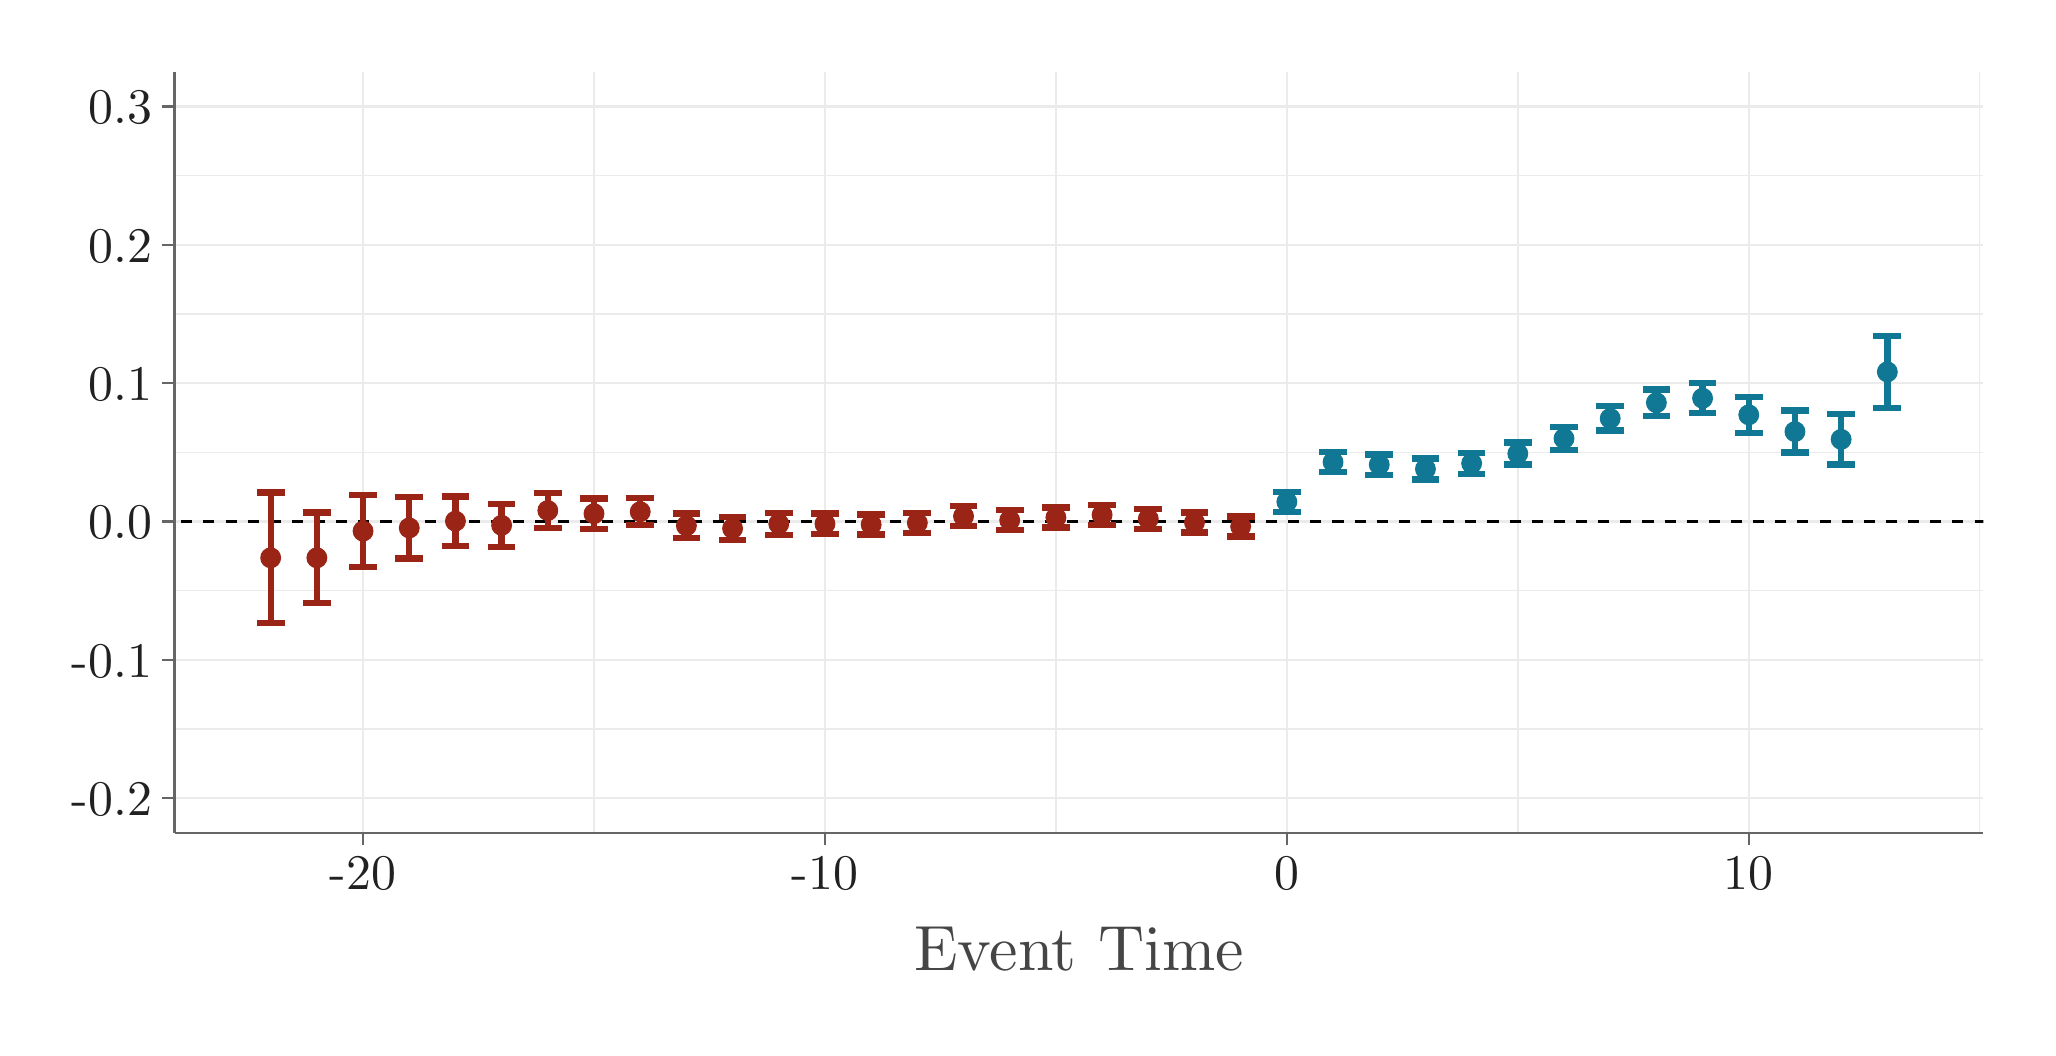
\begin{tikzpicture}[x=1pt,y=1pt]
\definecolor{fillColor}{RGB}{255,255,255}
\path[use as bounding box,fill=fillColor,fill opacity=0.00] (0,0) rectangle (722.70,361.35);
\begin{scope}
\path[clip] (  0.00,  0.00) rectangle (722.70,361.35);
\definecolor{fillColor}{RGB}{255,255,255}

\path[fill=fillColor] (  0.00, -0.00) rectangle (722.70,361.35);
\end{scope}
\begin{scope}
\path[clip] ( 53.09, 70.42) rectangle (706.70,345.35);
\definecolor{fillColor}{RGB}{255,255,255}

\path[fill=fillColor] ( 53.09, 70.42) rectangle (706.70,345.35);
\definecolor{drawColor}{gray}{0.92}

\path[draw=drawColor,line width= 0.5pt,line join=round] ( 53.09,107.91) --
	(706.70,107.91);

\path[draw=drawColor,line width= 0.5pt,line join=round] ( 53.09,157.90) --
	(706.70,157.90);

\path[draw=drawColor,line width= 0.5pt,line join=round] ( 53.09,207.89) --
	(706.70,207.89);

\path[draw=drawColor,line width= 0.5pt,line join=round] ( 53.09,257.87) --
	(706.70,257.87);

\path[draw=drawColor,line width= 0.5pt,line join=round] ( 53.09,307.86) --
	(706.70,307.86);

\path[draw=drawColor,line width= 0.5pt,line join=round] (204.64, 70.42) --
	(204.64,345.35);

\path[draw=drawColor,line width= 0.5pt,line join=round] (371.55, 70.42) --
	(371.55,345.35);

\path[draw=drawColor,line width= 0.5pt,line join=round] (538.46, 70.42) --
	(538.46,345.35);

\path[draw=drawColor,line width= 0.5pt,line join=round] (705.36, 70.42) --
	(705.36,345.35);

\path[draw=drawColor,line width= 0.9pt,line join=round] ( 53.09, 82.92) --
	(706.70, 82.92);

\path[draw=drawColor,line width= 0.9pt,line join=round] ( 53.09,132.91) --
	(706.70,132.91);

\path[draw=drawColor,line width= 0.9pt,line join=round] ( 53.09,182.89) --
	(706.70,182.89);

\path[draw=drawColor,line width= 0.9pt,line join=round] ( 53.09,232.88) --
	(706.70,232.88);

\path[draw=drawColor,line width= 0.9pt,line join=round] ( 53.09,282.87) --
	(706.70,282.87);

\path[draw=drawColor,line width= 0.9pt,line join=round] ( 53.09,332.85) --
	(706.70,332.85);

\path[draw=drawColor,line width= 0.9pt,line join=round] (121.19, 70.42) --
	(121.19,345.35);

\path[draw=drawColor,line width= 0.9pt,line join=round] (288.10, 70.42) --
	(288.10,345.35);

\path[draw=drawColor,line width= 0.9pt,line join=round] (455.00, 70.42) --
	(455.00,345.35);

\path[draw=drawColor,line width= 0.9pt,line join=round] (621.91, 70.42) --
	(621.91,345.35);
\definecolor{drawColor}{RGB}{0,0,0}

\path[draw=drawColor,line width= 0.9pt,dash pattern=on 4pt off 4pt ,line join=round] (-600.51,182.89) -- (1360.31,182.89);
\definecolor{drawColor}{RGB}{154,36,21}
\definecolor{fillColor}{RGB}{154,36,21}

\path[draw=drawColor,line width= 0.4pt,line join=round,line cap=round,fill=fillColor] ( 87.81,169.78) circle (  3.57);

\path[draw=drawColor,line width= 0.4pt,line join=round,line cap=round,fill=fillColor] (104.50,169.78) circle (  3.57);

\path[draw=drawColor,line width= 0.4pt,line join=round,line cap=round,fill=fillColor] (121.19,179.44) circle (  3.57);

\path[draw=drawColor,line width= 0.4pt,line join=round,line cap=round,fill=fillColor] (137.88,180.57) circle (  3.57);

\path[draw=drawColor,line width= 0.4pt,line join=round,line cap=round,fill=fillColor] (154.57,183.04) circle (  3.57);

\path[draw=drawColor,line width= 0.4pt,line join=round,line cap=round,fill=fillColor] (171.26,181.53) circle (  3.57);

\path[draw=drawColor,line width= 0.4pt,line join=round,line cap=round,fill=fillColor] (187.95,186.86) circle (  3.57);

\path[draw=drawColor,line width= 0.4pt,line join=round,line cap=round,fill=fillColor] (204.64,185.73) circle (  3.57);

\path[draw=drawColor,line width= 0.4pt,line join=round,line cap=round,fill=fillColor] (221.34,186.43) circle (  3.57);

\path[draw=drawColor,line width= 0.4pt,line join=round,line cap=round,fill=fillColor] (238.03,181.37) circle (  3.57);

\path[draw=drawColor,line width= 0.4pt,line join=round,line cap=round,fill=fillColor] (254.72,180.39) circle (  3.57);

\path[draw=drawColor,line width= 0.4pt,line join=round,line cap=round,fill=fillColor] (271.41,182.05) circle (  3.57);

\path[draw=drawColor,line width= 0.4pt,line join=round,line cap=round,fill=fillColor] (288.10,182.05) circle (  3.57);

\path[draw=drawColor,line width= 0.4pt,line join=round,line cap=round,fill=fillColor] (304.79,181.79) circle (  3.57);

\path[draw=drawColor,line width= 0.4pt,line join=round,line cap=round,fill=fillColor] (321.48,182.38) circle (  3.57);

\path[draw=drawColor,line width= 0.4pt,line join=round,line cap=round,fill=fillColor] (338.17,184.80) circle (  3.57);

\path[draw=drawColor,line width= 0.4pt,line join=round,line cap=round,fill=fillColor] (354.86,183.35) circle (  3.57);

\path[draw=drawColor,line width= 0.4pt,line join=round,line cap=round,fill=fillColor] (371.55,184.33) circle (  3.57);

\path[draw=drawColor,line width= 0.4pt,line join=round,line cap=round,fill=fillColor] (388.24,185.30) circle (  3.57);

\path[draw=drawColor,line width= 0.4pt,line join=round,line cap=round,fill=fillColor] (404.93,183.86) circle (  3.57);

\path[draw=drawColor,line width= 0.4pt,line join=round,line cap=round,fill=fillColor] (421.62,182.57) circle (  3.57);

\path[draw=drawColor,line width= 0.4pt,line join=round,line cap=round,fill=fillColor] (438.31,181.13) circle (  3.57);
\definecolor{drawColor}{RGB}{16,120,149}
\definecolor{fillColor}{RGB}{16,120,149}

\path[draw=drawColor,line width= 0.4pt,line join=round,line cap=round,fill=fillColor] (455.00,190.01) circle (  3.57);

\path[draw=drawColor,line width= 0.4pt,line join=round,line cap=round,fill=fillColor] (471.70,204.36) circle (  3.57);

\path[draw=drawColor,line width= 0.4pt,line join=round,line cap=round,fill=fillColor] (488.39,203.45) circle (  3.57);

\path[draw=drawColor,line width= 0.4pt,line join=round,line cap=round,fill=fillColor] (505.08,201.88) circle (  3.57);

\path[draw=drawColor,line width= 0.4pt,line join=round,line cap=round,fill=fillColor] (521.77,203.90) circle (  3.57);

\path[draw=drawColor,line width= 0.4pt,line join=round,line cap=round,fill=fillColor] (538.46,207.43) circle (  3.57);

\path[draw=drawColor,line width= 0.4pt,line join=round,line cap=round,fill=fillColor] (555.15,212.88) circle (  3.57);

\path[draw=drawColor,line width= 0.4pt,line join=round,line cap=round,fill=fillColor] (571.84,220.14) circle (  3.57);

\path[draw=drawColor,line width= 0.4pt,line join=round,line cap=round,fill=fillColor] (588.53,225.83) circle (  3.57);

\path[draw=drawColor,line width= 0.4pt,line join=round,line cap=round,fill=fillColor] (605.22,227.45) circle (  3.57);

\path[draw=drawColor,line width= 0.4pt,line join=round,line cap=round,fill=fillColor] (621.91,221.44) circle (  3.57);

\path[draw=drawColor,line width= 0.4pt,line join=round,line cap=round,fill=fillColor] (638.60,215.37) circle (  3.57);

\path[draw=drawColor,line width= 0.4pt,line join=round,line cap=round,fill=fillColor] (655.29,212.59) circle (  3.57);

\path[draw=drawColor,line width= 0.4pt,line join=round,line cap=round,fill=fillColor] (671.98,236.96) circle (  3.57);
\definecolor{drawColor}{RGB}{154,36,21}

\path[draw=drawColor,line width= 2.3pt,line join=round] ( 82.80,193.38) --
	( 92.82,193.38);

\path[draw=drawColor,line width= 2.3pt,line join=round] ( 87.81,193.38) --
	( 87.81,146.17);

\path[draw=drawColor,line width= 2.3pt,line join=round] ( 82.80,146.17) --
	( 92.82,146.17);

\path[draw=drawColor,line width= 2.3pt,line join=round] ( 99.49,186.09) --
	(109.51,186.09);

\path[draw=drawColor,line width= 2.3pt,line join=round] (104.50,186.09) --
	(104.50,153.47);

\path[draw=drawColor,line width= 2.3pt,line join=round] ( 99.49,153.47) --
	(109.51,153.47);

\path[draw=drawColor,line width= 2.3pt,line join=round] (116.18,192.37) --
	(126.20,192.37);

\path[draw=drawColor,line width= 2.3pt,line join=round] (121.19,192.37) --
	(121.19,166.51);

\path[draw=drawColor,line width= 2.3pt,line join=round] (116.18,166.51) --
	(126.20,166.51);

\path[draw=drawColor,line width= 2.3pt,line join=round] (132.87,191.67) --
	(142.89,191.67);

\path[draw=drawColor,line width= 2.3pt,line join=round] (137.88,191.67) --
	(137.88,169.47);

\path[draw=drawColor,line width= 2.3pt,line join=round] (132.87,169.47) --
	(142.89,169.47);

\path[draw=drawColor,line width= 2.3pt,line join=round] (149.57,191.94) --
	(159.58,191.94);

\path[draw=drawColor,line width= 2.3pt,line join=round] (154.57,191.94) --
	(154.57,174.15);

\path[draw=drawColor,line width= 2.3pt,line join=round] (149.57,174.15) --
	(159.58,174.15);

\path[draw=drawColor,line width= 2.3pt,line join=round] (166.26,189.26) --
	(176.27,189.26);

\path[draw=drawColor,line width= 2.3pt,line join=round] (171.26,189.26) --
	(171.26,173.80);

\path[draw=drawColor,line width= 2.3pt,line join=round] (166.26,173.80) --
	(176.27,173.80);

\path[draw=drawColor,line width= 2.3pt,line join=round] (182.95,193.16) --
	(192.96,193.16);

\path[draw=drawColor,line width= 2.3pt,line join=round] (187.95,193.16) --
	(187.95,180.55);

\path[draw=drawColor,line width= 2.3pt,line join=round] (182.95,180.55) --
	(192.96,180.55);

\path[draw=drawColor,line width= 2.3pt,line join=round] (199.64,191.27) --
	(209.65,191.27);

\path[draw=drawColor,line width= 2.3pt,line join=round] (204.64,191.27) --
	(204.64,180.20);

\path[draw=drawColor,line width= 2.3pt,line join=round] (199.64,180.20) --
	(209.65,180.20);

\path[draw=drawColor,line width= 2.3pt,line join=round] (216.33,191.29) --
	(226.34,191.29);

\path[draw=drawColor,line width= 2.3pt,line join=round] (221.34,191.29) --
	(221.34,181.57);

\path[draw=drawColor,line width= 2.3pt,line join=round] (216.33,181.57) --
	(226.34,181.57);

\path[draw=drawColor,line width= 2.3pt,line join=round] (233.02,185.74) --
	(243.03,185.74);

\path[draw=drawColor,line width= 2.3pt,line join=round] (238.03,185.74) --
	(238.03,177.00);

\path[draw=drawColor,line width= 2.3pt,line join=round] (233.02,177.00) --
	(243.03,177.00);

\path[draw=drawColor,line width= 2.3pt,line join=round] (249.71,184.51) --
	(259.72,184.51);

\path[draw=drawColor,line width= 2.3pt,line join=round] (254.72,184.51) --
	(254.72,176.27);

\path[draw=drawColor,line width= 2.3pt,line join=round] (249.71,176.27) --
	(259.72,176.27);

\path[draw=drawColor,line width= 2.3pt,line join=round] (266.40,186.01) --
	(276.41,186.01);

\path[draw=drawColor,line width= 2.3pt,line join=round] (271.41,186.01) --
	(271.41,178.10);

\path[draw=drawColor,line width= 2.3pt,line join=round] (266.40,178.10) --
	(276.41,178.10);

\path[draw=drawColor,line width= 2.3pt,line join=round] (283.09,185.82) --
	(293.10,185.82);

\path[draw=drawColor,line width= 2.3pt,line join=round] (288.10,185.82) --
	(288.10,178.28);

\path[draw=drawColor,line width= 2.3pt,line join=round] (283.09,178.28) --
	(293.10,178.28);

\path[draw=drawColor,line width= 2.3pt,line join=round] (299.78,185.42) --
	(309.80,185.42);

\path[draw=drawColor,line width= 2.3pt,line join=round] (304.79,185.42) --
	(304.79,178.17);

\path[draw=drawColor,line width= 2.3pt,line join=round] (299.78,178.17) --
	(309.80,178.17);

\path[draw=drawColor,line width= 2.3pt,line join=round] (316.47,186.00) --
	(326.49,186.00);

\path[draw=drawColor,line width= 2.3pt,line join=round] (321.48,186.00) --
	(321.48,178.76);

\path[draw=drawColor,line width= 2.3pt,line join=round] (316.47,178.76) --
	(326.49,178.76);

\path[draw=drawColor,line width= 2.3pt,line join=round] (333.16,188.42) --
	(343.18,188.42);

\path[draw=drawColor,line width= 2.3pt,line join=round] (338.17,188.42) --
	(338.17,181.18);

\path[draw=drawColor,line width= 2.3pt,line join=round] (333.16,181.18) --
	(343.18,181.18);

\path[draw=drawColor,line width= 2.3pt,line join=round] (349.85,186.97) --
	(359.87,186.97);

\path[draw=drawColor,line width= 2.3pt,line join=round] (354.86,186.97) --
	(354.86,179.73);

\path[draw=drawColor,line width= 2.3pt,line join=round] (349.85,179.73) --
	(359.87,179.73);

\path[draw=drawColor,line width= 2.3pt,line join=round] (366.54,187.95) --
	(376.56,187.95);

\path[draw=drawColor,line width= 2.3pt,line join=round] (371.55,187.95) --
	(371.55,180.71);

\path[draw=drawColor,line width= 2.3pt,line join=round] (366.54,180.71) --
	(376.56,180.71);

\path[draw=drawColor,line width= 2.3pt,line join=round] (383.23,188.92) --
	(393.25,188.92);

\path[draw=drawColor,line width= 2.3pt,line join=round] (388.24,188.92) --
	(388.24,181.68);

\path[draw=drawColor,line width= 2.3pt,line join=round] (383.23,181.68) --
	(393.25,181.68);

\path[draw=drawColor,line width= 2.3pt,line join=round] (399.93,187.48) --
	(409.94,187.48);

\path[draw=drawColor,line width= 2.3pt,line join=round] (404.93,187.48) --
	(404.93,180.23);

\path[draw=drawColor,line width= 2.3pt,line join=round] (399.93,180.23) --
	(409.94,180.23);

\path[draw=drawColor,line width= 2.3pt,line join=round] (416.62,186.19) --
	(426.63,186.19);

\path[draw=drawColor,line width= 2.3pt,line join=round] (421.62,186.19) --
	(421.62,178.95);

\path[draw=drawColor,line width= 2.3pt,line join=round] (416.62,178.95) --
	(426.63,178.95);

\path[draw=drawColor,line width= 2.3pt,line join=round] (433.31,184.75) --
	(443.32,184.75);

\path[draw=drawColor,line width= 2.3pt,line join=round] (438.31,184.75) --
	(438.31,177.51);

\path[draw=drawColor,line width= 2.3pt,line join=round] (433.31,177.51) --
	(443.32,177.51);
\definecolor{drawColor}{RGB}{16,120,149}

\path[draw=drawColor,line width= 2.3pt,line join=round] (450.00,193.63) --
	(460.01,193.63);

\path[draw=drawColor,line width= 2.3pt,line join=round] (455.00,193.63) --
	(455.00,186.39);

\path[draw=drawColor,line width= 2.3pt,line join=round] (450.00,186.39) --
	(460.01,186.39);

\path[draw=drawColor,line width= 2.3pt,line join=round] (466.69,208.03) --
	(476.70,208.03);

\path[draw=drawColor,line width= 2.3pt,line join=round] (471.70,208.03) --
	(471.70,200.70);

\path[draw=drawColor,line width= 2.3pt,line join=round] (466.69,200.70) --
	(476.70,200.70);

\path[draw=drawColor,line width= 2.3pt,line join=round] (483.38,207.16) --
	(493.39,207.16);

\path[draw=drawColor,line width= 2.3pt,line join=round] (488.39,207.16) --
	(488.39,199.74);

\path[draw=drawColor,line width= 2.3pt,line join=round] (483.38,199.74) --
	(493.39,199.74);

\path[draw=drawColor,line width= 2.3pt,line join=round] (500.07,205.66) --
	(510.08,205.66);

\path[draw=drawColor,line width= 2.3pt,line join=round] (505.08,205.66) --
	(505.08,198.11);

\path[draw=drawColor,line width= 2.3pt,line join=round] (500.07,198.11) --
	(510.08,198.11);

\path[draw=drawColor,line width= 2.3pt,line join=round] (516.76,207.73) --
	(526.77,207.73);

\path[draw=drawColor,line width= 2.3pt,line join=round] (521.77,207.73) --
	(521.77,200.07);

\path[draw=drawColor,line width= 2.3pt,line join=round] (516.76,200.07) --
	(526.77,200.07);

\path[draw=drawColor,line width= 2.3pt,line join=round] (533.45,211.40) --
	(543.47,211.40);

\path[draw=drawColor,line width= 2.3pt,line join=round] (538.46,211.40) --
	(538.46,203.47);

\path[draw=drawColor,line width= 2.3pt,line join=round] (533.45,203.47) --
	(543.47,203.47);

\path[draw=drawColor,line width= 2.3pt,line join=round] (550.14,216.98) --
	(560.16,216.98);

\path[draw=drawColor,line width= 2.3pt,line join=round] (555.15,216.98) --
	(555.15,208.78);

\path[draw=drawColor,line width= 2.3pt,line join=round] (550.14,208.78) --
	(560.16,208.78);

\path[draw=drawColor,line width= 2.3pt,line join=round] (566.83,224.56) --
	(576.85,224.56);

\path[draw=drawColor,line width= 2.3pt,line join=round] (571.84,224.56) --
	(571.84,215.72);

\path[draw=drawColor,line width= 2.3pt,line join=round] (566.83,215.72) --
	(576.85,215.72);

\path[draw=drawColor,line width= 2.3pt,line join=round] (583.52,230.62) --
	(593.54,230.62);

\path[draw=drawColor,line width= 2.3pt,line join=round] (588.53,230.62) --
	(588.53,221.04);

\path[draw=drawColor,line width= 2.3pt,line join=round] (583.52,221.04) --
	(593.54,221.04);

\path[draw=drawColor,line width= 2.3pt,line join=round] (600.21,232.87) --
	(610.23,232.87);

\path[draw=drawColor,line width= 2.3pt,line join=round] (605.22,232.87) --
	(605.22,222.02);

\path[draw=drawColor,line width= 2.3pt,line join=round] (600.21,222.02) --
	(610.23,222.02);

\path[draw=drawColor,line width= 2.3pt,line join=round] (616.90,227.90) --
	(626.92,227.90);

\path[draw=drawColor,line width= 2.3pt,line join=round] (621.91,227.90) --
	(621.91,214.97);

\path[draw=drawColor,line width= 2.3pt,line join=round] (616.90,214.97) --
	(626.92,214.97);

\path[draw=drawColor,line width= 2.3pt,line join=round] (633.59,222.97) --
	(643.61,222.97);

\path[draw=drawColor,line width= 2.3pt,line join=round] (638.60,222.97) --
	(638.60,207.78);

\path[draw=drawColor,line width= 2.3pt,line join=round] (633.59,207.78) --
	(643.61,207.78);

\path[draw=drawColor,line width= 2.3pt,line join=round] (650.29,221.64) --
	(660.30,221.64);

\path[draw=drawColor,line width= 2.3pt,line join=round] (655.29,221.64) --
	(655.29,203.55);

\path[draw=drawColor,line width= 2.3pt,line join=round] (650.29,203.55) --
	(660.30,203.55);

\path[draw=drawColor,line width= 2.3pt,line join=round] (666.98,249.99) --
	(676.99,249.99);

\path[draw=drawColor,line width= 2.3pt,line join=round] (671.98,249.99) --
	(671.98,223.94);

\path[draw=drawColor,line width= 2.3pt,line join=round] (666.98,223.94) --
	(676.99,223.94);

\path[] ( 53.09, 70.42) rectangle (706.70,345.35);
\end{scope}
\begin{scope}
\path[clip] (  0.00,  0.00) rectangle (722.70,361.35);
\definecolor{drawColor}{gray}{0.40}

\path[draw=drawColor,line width= 0.9pt,line join=round] ( 53.09, 70.42) --
	( 53.09,345.35);
\end{scope}
\begin{scope}
\path[clip] (  0.00,  0.00) rectangle (722.70,361.35);
\definecolor{drawColor}{gray}{0.13}

\node[text=drawColor,anchor=base east,inner sep=0pt, outer sep=0pt, scale=  1.80] at ( 44.99, 76.72) {-0.2};

\node[text=drawColor,anchor=base east,inner sep=0pt, outer sep=0pt, scale=  1.80] at ( 44.99,126.71) {-0.1};

\node[text=drawColor,anchor=base east,inner sep=0pt, outer sep=0pt, scale=  1.80] at ( 44.99,176.69) {0.0};

\node[text=drawColor,anchor=base east,inner sep=0pt, outer sep=0pt, scale=  1.80] at ( 44.99,226.68) {0.1};

\node[text=drawColor,anchor=base east,inner sep=0pt, outer sep=0pt, scale=  1.80] at ( 44.99,276.67) {0.2};

\node[text=drawColor,anchor=base east,inner sep=0pt, outer sep=0pt, scale=  1.80] at ( 44.99,326.65) {0.3};
\end{scope}
\begin{scope}
\path[clip] (  0.00,  0.00) rectangle (722.70,361.35);
\definecolor{drawColor}{gray}{0.40}

\path[draw=drawColor,line width= 0.9pt,line join=round] ( 48.59, 82.92) --
	( 53.09, 82.92);

\path[draw=drawColor,line width= 0.9pt,line join=round] ( 48.59,132.91) --
	( 53.09,132.91);

\path[draw=drawColor,line width= 0.9pt,line join=round] ( 48.59,182.89) --
	( 53.09,182.89);

\path[draw=drawColor,line width= 0.9pt,line join=round] ( 48.59,232.88) --
	( 53.09,232.88);

\path[draw=drawColor,line width= 0.9pt,line join=round] ( 48.59,282.87) --
	( 53.09,282.87);

\path[draw=drawColor,line width= 0.9pt,line join=round] ( 48.59,332.85) --
	( 53.09,332.85);
\end{scope}
\begin{scope}
\path[clip] (  0.00,  0.00) rectangle (722.70,361.35);
\definecolor{drawColor}{gray}{0.40}

\path[draw=drawColor,line width= 0.9pt,line join=round] ( 53.09, 70.42) --
	(706.70, 70.42);
\end{scope}
\begin{scope}
\path[clip] (  0.00,  0.00) rectangle (722.70,361.35);
\definecolor{drawColor}{gray}{0.40}

\path[draw=drawColor,line width= 0.9pt,line join=round] (121.19, 65.92) --
	(121.19, 70.42);

\path[draw=drawColor,line width= 0.9pt,line join=round] (288.10, 65.92) --
	(288.10, 70.42);

\path[draw=drawColor,line width= 0.9pt,line join=round] (455.00, 65.92) --
	(455.00, 70.42);

\path[draw=drawColor,line width= 0.9pt,line join=round] (621.91, 65.92) --
	(621.91, 70.42);
\end{scope}
\begin{scope}
\path[clip] (  0.00,  0.00) rectangle (722.70,361.35);
\definecolor{drawColor}{gray}{0.13}

\node[text=drawColor,anchor=base,inner sep=0pt, outer sep=0pt, scale=  1.80] at (121.19, 49.93) {-20};

\node[text=drawColor,anchor=base,inner sep=0pt, outer sep=0pt, scale=  1.80] at (288.10, 49.93) {-10};

\node[text=drawColor,anchor=base,inner sep=0pt, outer sep=0pt, scale=  1.80] at (455.00, 49.93) {0};

\node[text=drawColor,anchor=base,inner sep=0pt, outer sep=0pt, scale=  1.80] at (621.91, 49.93) {10};
\end{scope}
\begin{scope}
\path[clip] (  0.00,  0.00) rectangle (722.70,361.35);
\definecolor{drawColor}{gray}{0.27}

\node[text=drawColor,anchor=base,inner sep=0pt, outer sep=0pt, scale=  2.31] at (379.90, 20.50) {Event Time};
\end{scope}
\end{tikzpicture}
